% Options for packages loaded elsewhere
\PassOptionsToPackage{unicode}{hyperref}
\PassOptionsToPackage{hyphens}{url}
%
\documentclass[
]{article}
\usepackage{amsmath,amssymb}
\usepackage{lmodern}
\usepackage{iftex}
\ifPDFTeX
  \usepackage[T1]{fontenc}
  \usepackage[utf8]{inputenc}
  \usepackage{textcomp} % provide euro and other symbols
\else % if luatex or xetex
  \usepackage{unicode-math}
  \defaultfontfeatures{Scale=MatchLowercase}
  \defaultfontfeatures[\rmfamily]{Ligatures=TeX,Scale=1}
\fi
% Use upquote if available, for straight quotes in verbatim environments
\IfFileExists{upquote.sty}{\usepackage{upquote}}{}
\IfFileExists{microtype.sty}{% use microtype if available
  \usepackage[]{microtype}
  \UseMicrotypeSet[protrusion]{basicmath} % disable protrusion for tt fonts
}{}
\makeatletter
\@ifundefined{KOMAClassName}{% if non-KOMA class
  \IfFileExists{parskip.sty}{%
    \usepackage{parskip}
  }{% else
    \setlength{\parindent}{0pt}
    \setlength{\parskip}{6pt plus 2pt minus 1pt}}
}{% if KOMA class
  \KOMAoptions{parskip=half}}
\makeatother
\usepackage{xcolor}
\usepackage{longtable,booktabs,array}
\usepackage{multirow}
\usepackage{calc} % for calculating minipage widths
% Correct order of tables after \paragraph or \subparagraph
\usepackage{etoolbox}
\makeatletter
\patchcmd\longtable{\par}{\if@noskipsec\mbox{}\fi\par}{}{}
\makeatother
% Allow footnotes in longtable head/foot
\IfFileExists{footnotehyper.sty}{\usepackage{footnotehyper}}{\usepackage{footnote}}
\makesavenoteenv{longtable}
\usepackage{graphicx}
\makeatletter
\def\maxwidth{\ifdim\Gin@nat@width>\linewidth\linewidth\else\Gin@nat@width\fi}
\def\maxheight{\ifdim\Gin@nat@height>\textheight\textheight\else\Gin@nat@height\fi}
\makeatother
% Scale images if necessary, so that they will not overflow the page
% margins by default, and it is still possible to overwrite the defaults
% using explicit options in \includegraphics[width, height, ...]{}
\setkeys{Gin}{width=\maxwidth,height=\maxheight,keepaspectratio}
% Set default figure placement to htbp
\makeatletter
\def\fps@figure{htbp}
\makeatother
\usepackage[normalem]{ulem}
\setlength{\emergencystretch}{3em} % prevent overfull lines
\providecommand{\tightlist}{%
  \setlength{\itemsep}{0pt}\setlength{\parskip}{0pt}}
\setcounter{secnumdepth}{-\maxdimen} % remove section numbering
\ifLuaTeX
  \usepackage{selnolig}  % disable illegal ligatures
\fi
\IfFileExists{bookmark.sty}{\usepackage{bookmark}}{\usepackage{hyperref}}
\IfFileExists{xurl.sty}{\usepackage{xurl}}{} % add URL line breaks if available
\urlstyle{same} % disable monospaced font for URLs
\hypersetup{
  hidelinks,
  pdfcreator={LaTeX via pandoc}}

\author{}
\date{}

\begin{document}

\emph{\textbf{Chapter 1 -- The Engineering Design Process}}

\textbf{1.In your own words, describe the difference between
prescriptive and descriptive design} \textbf{processes. Cite examples of
each. {[}R{]}}

\begin{quote}
Prescriptive design processes ``prescribe'' an exact sequence of steps
and decisions for realizing a design. There are often decisions that
must be made in prescriptive processes for determining whether to move
from one stage to the next, or to move to the next phase. Descriptive
processes describe the general steps needed to achieve a design, but do
not explicitly layout the steps which should be followed to achieve the
design.
\end{quote}

\textbf{2.Describe the relationship between the Problem Identification,
Research, and} \textbf{Requirements Specification phases of the design
process. {[}R/A{]}}

\begin{quote}
Problem Identification, Research, and Requirements Specification are
three early phases of the design process. The overall objective of these
phases is to identify a problem, analyze it, and develop requirements
for its solution. The Problem ID phase is where the end-user needs are
determined, while further analysis occurs in the research phase. Both
problem and research phases are used to develop a Requirements
Specification that provides the requirements for those elements that
must be satisfied in order for a successful design.
\end{quote}

\textbf{3.Describe the relationship between the Concept Generation and
Design phases of the} \textbf{design process. {[}R/A{]}}

\begin{quote}
In Concept Generation, different technical options for solving the
design are given -- one is selected to pursue. In the Design Phase, the
option selected from Concept Generation is further clarified and the
design architecture is more clearly defined.
\end{quote}

\textbf{4.Construct a prescriptive design process for the Problem
Identification, Research, Specification, Concept, and Design phases of
the design process. The result should be a flow chart that contains
decision blocks and iteration as necessary. {[}A{]}}

\begin{quote}
In the prescriptive design process, shown in the figure below, there are
two decision points, one of which occurs after the requirements are
determined. The objective in this decision is to determine whether the
requirements satisfy the end-user needs. If not, the needs must be
re-examined and the requirements must be updated as necessary, in order
to meet the customer needs. The other decision occurs after the design
is generated. Here, the objective is to determine if the design
satisfies the requirements. If not, a new design concept must be
generated.

\emph{\textbf{Note:} This is only one possible solution, and there are
certainly other possible design processes that could be developed.}
\end{quote}

1


\includegraphics[width=0.22083in,height=0.1291in]{vertopal_51ee0767b0954baa94830c5e62d37958/media/image5.png}
\includegraphics[width=0.63333in,height=0.62295in]{vertopal_51ee0767b0954baa94830c5e62d37958/media/image6.png}
\includegraphics[width=\textwidth,height=0.46884in]{vertopal_51ee0767b0954baa94830c5e62d37958/media/image7.png}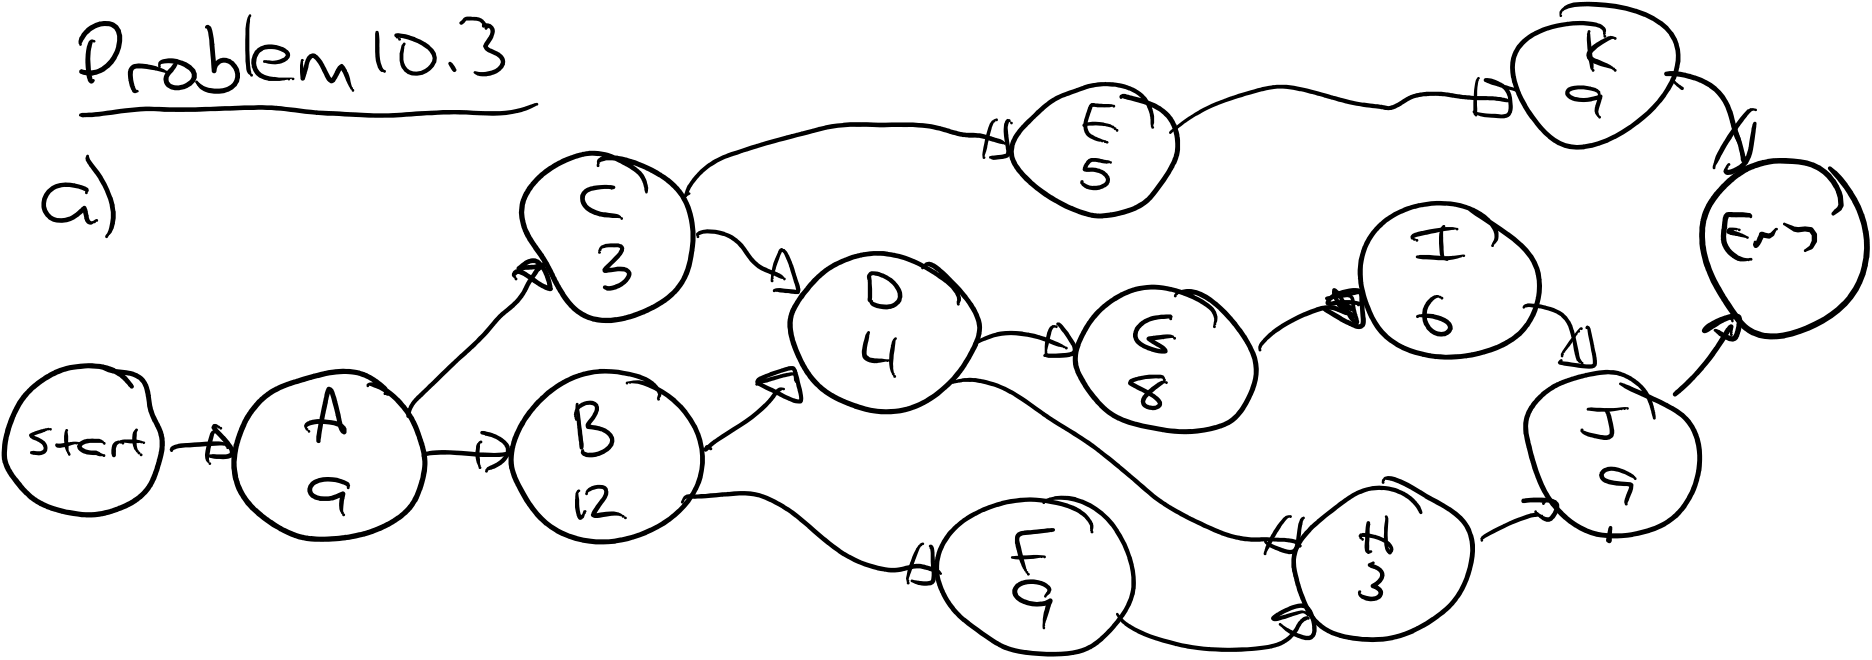
\includegraphics[width=0.63472in,height=0.35186in]{vertopal_51ee0767b0954baa94830c5e62d37958/media/image8.png}
\includegraphics[width=0.18056in,height=0.47222in]{vertopal_51ee0767b0954baa94830c5e62d37958/media/image9.png}
\includegraphics[width=0.14028in,height=0.46873in]{vertopal_51ee0767b0954baa94830c5e62d37958/media/image10.png}
\includegraphics[width=0.14028in,height=0.46873in]{vertopal_51ee0767b0954baa94830c5e62d37958/media/image10.png}
\includegraphics[width=0.36667in,height=0.2433in]{vertopal_51ee0767b0954baa94830c5e62d37958/media/image11.png}
\includegraphics[width=0.17361in,height=0.24169in]{vertopal_51ee0767b0954baa94830c5e62d37958/media/image12.png}
\includegraphics[width=0.36667in,height=0.2433in]{vertopal_51ee0767b0954baa94830c5e62d37958/media/image13.png}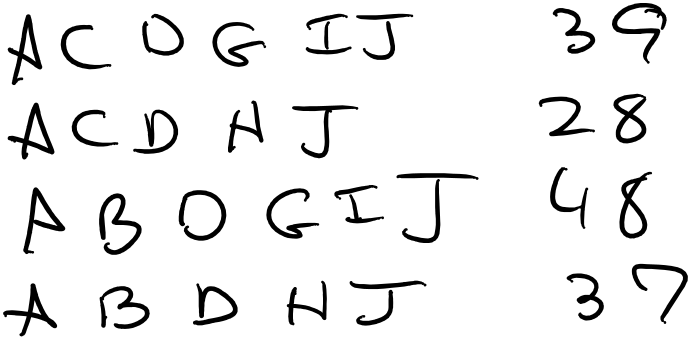
\includegraphics[width=\textwidth,height=0.24036in]{vertopal_51ee0767b0954baa94830c5e62d37958/media/image14.png}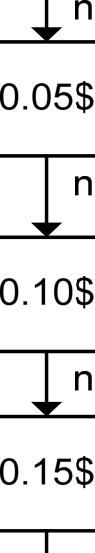
\includegraphics[width=0.63333in,height=0.34954in]{vertopal_51ee0767b0954baa94830c5e62d37958/media/image15.png}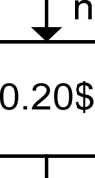
\includegraphics[width=0.7in,height=0.13168in]{vertopal_51ee0767b0954baa94830c5e62d37958/media/image16.png}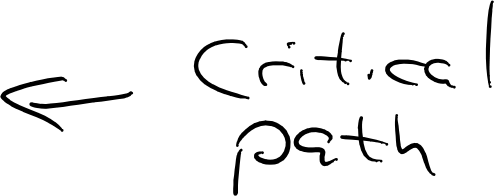
\includegraphics[width=0.2875in,height=0.31867in]{vertopal_51ee0767b0954baa94830c5e62d37958/media/image17.png}
\includegraphics[width=\textwidth,height=0.28504in]{vertopal_51ee0767b0954baa94830c5e62d37958/media/image18.png}
\includegraphics[width=1.59722in,height=7.27778in]{vertopal_51ee0767b0954baa94830c5e62d37958/media/image19.png}

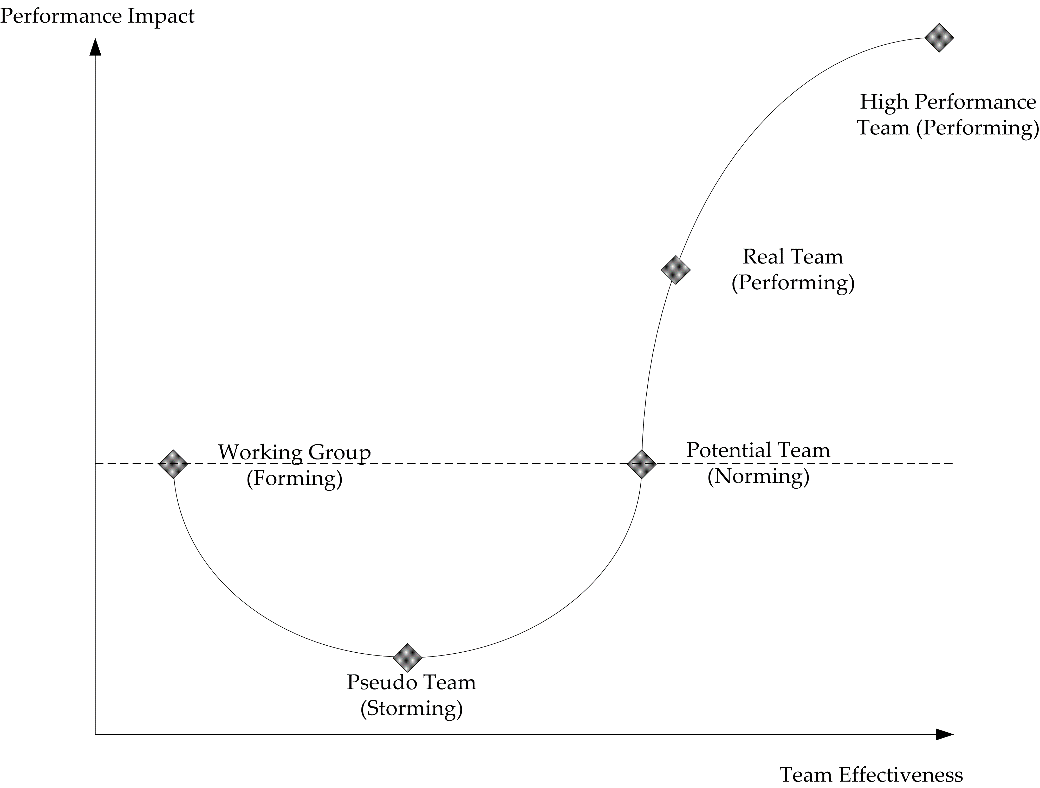
\includegraphics[width=0.60694in,height=0.15in]{vertopal_51ee0767b0954baa94830c5e62d37958/media/image1.png}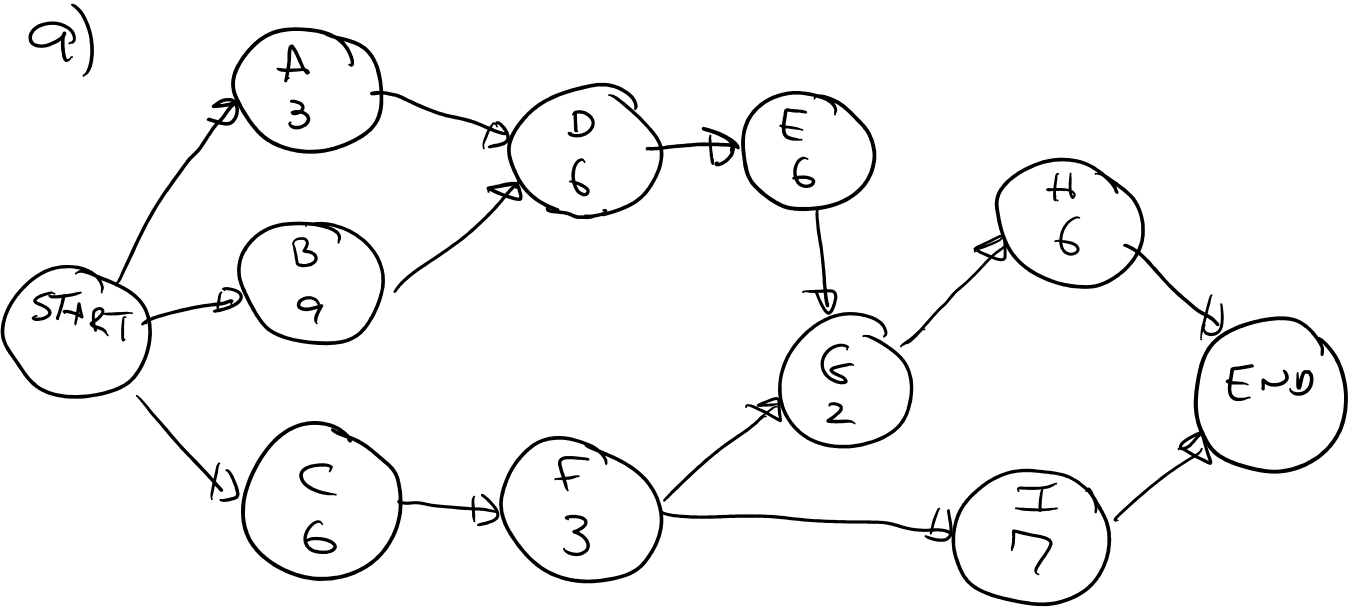
\includegraphics[width=0.2875in,height=0.15in]{vertopal_51ee0767b0954baa94830c5e62d37958/media/image2.png}

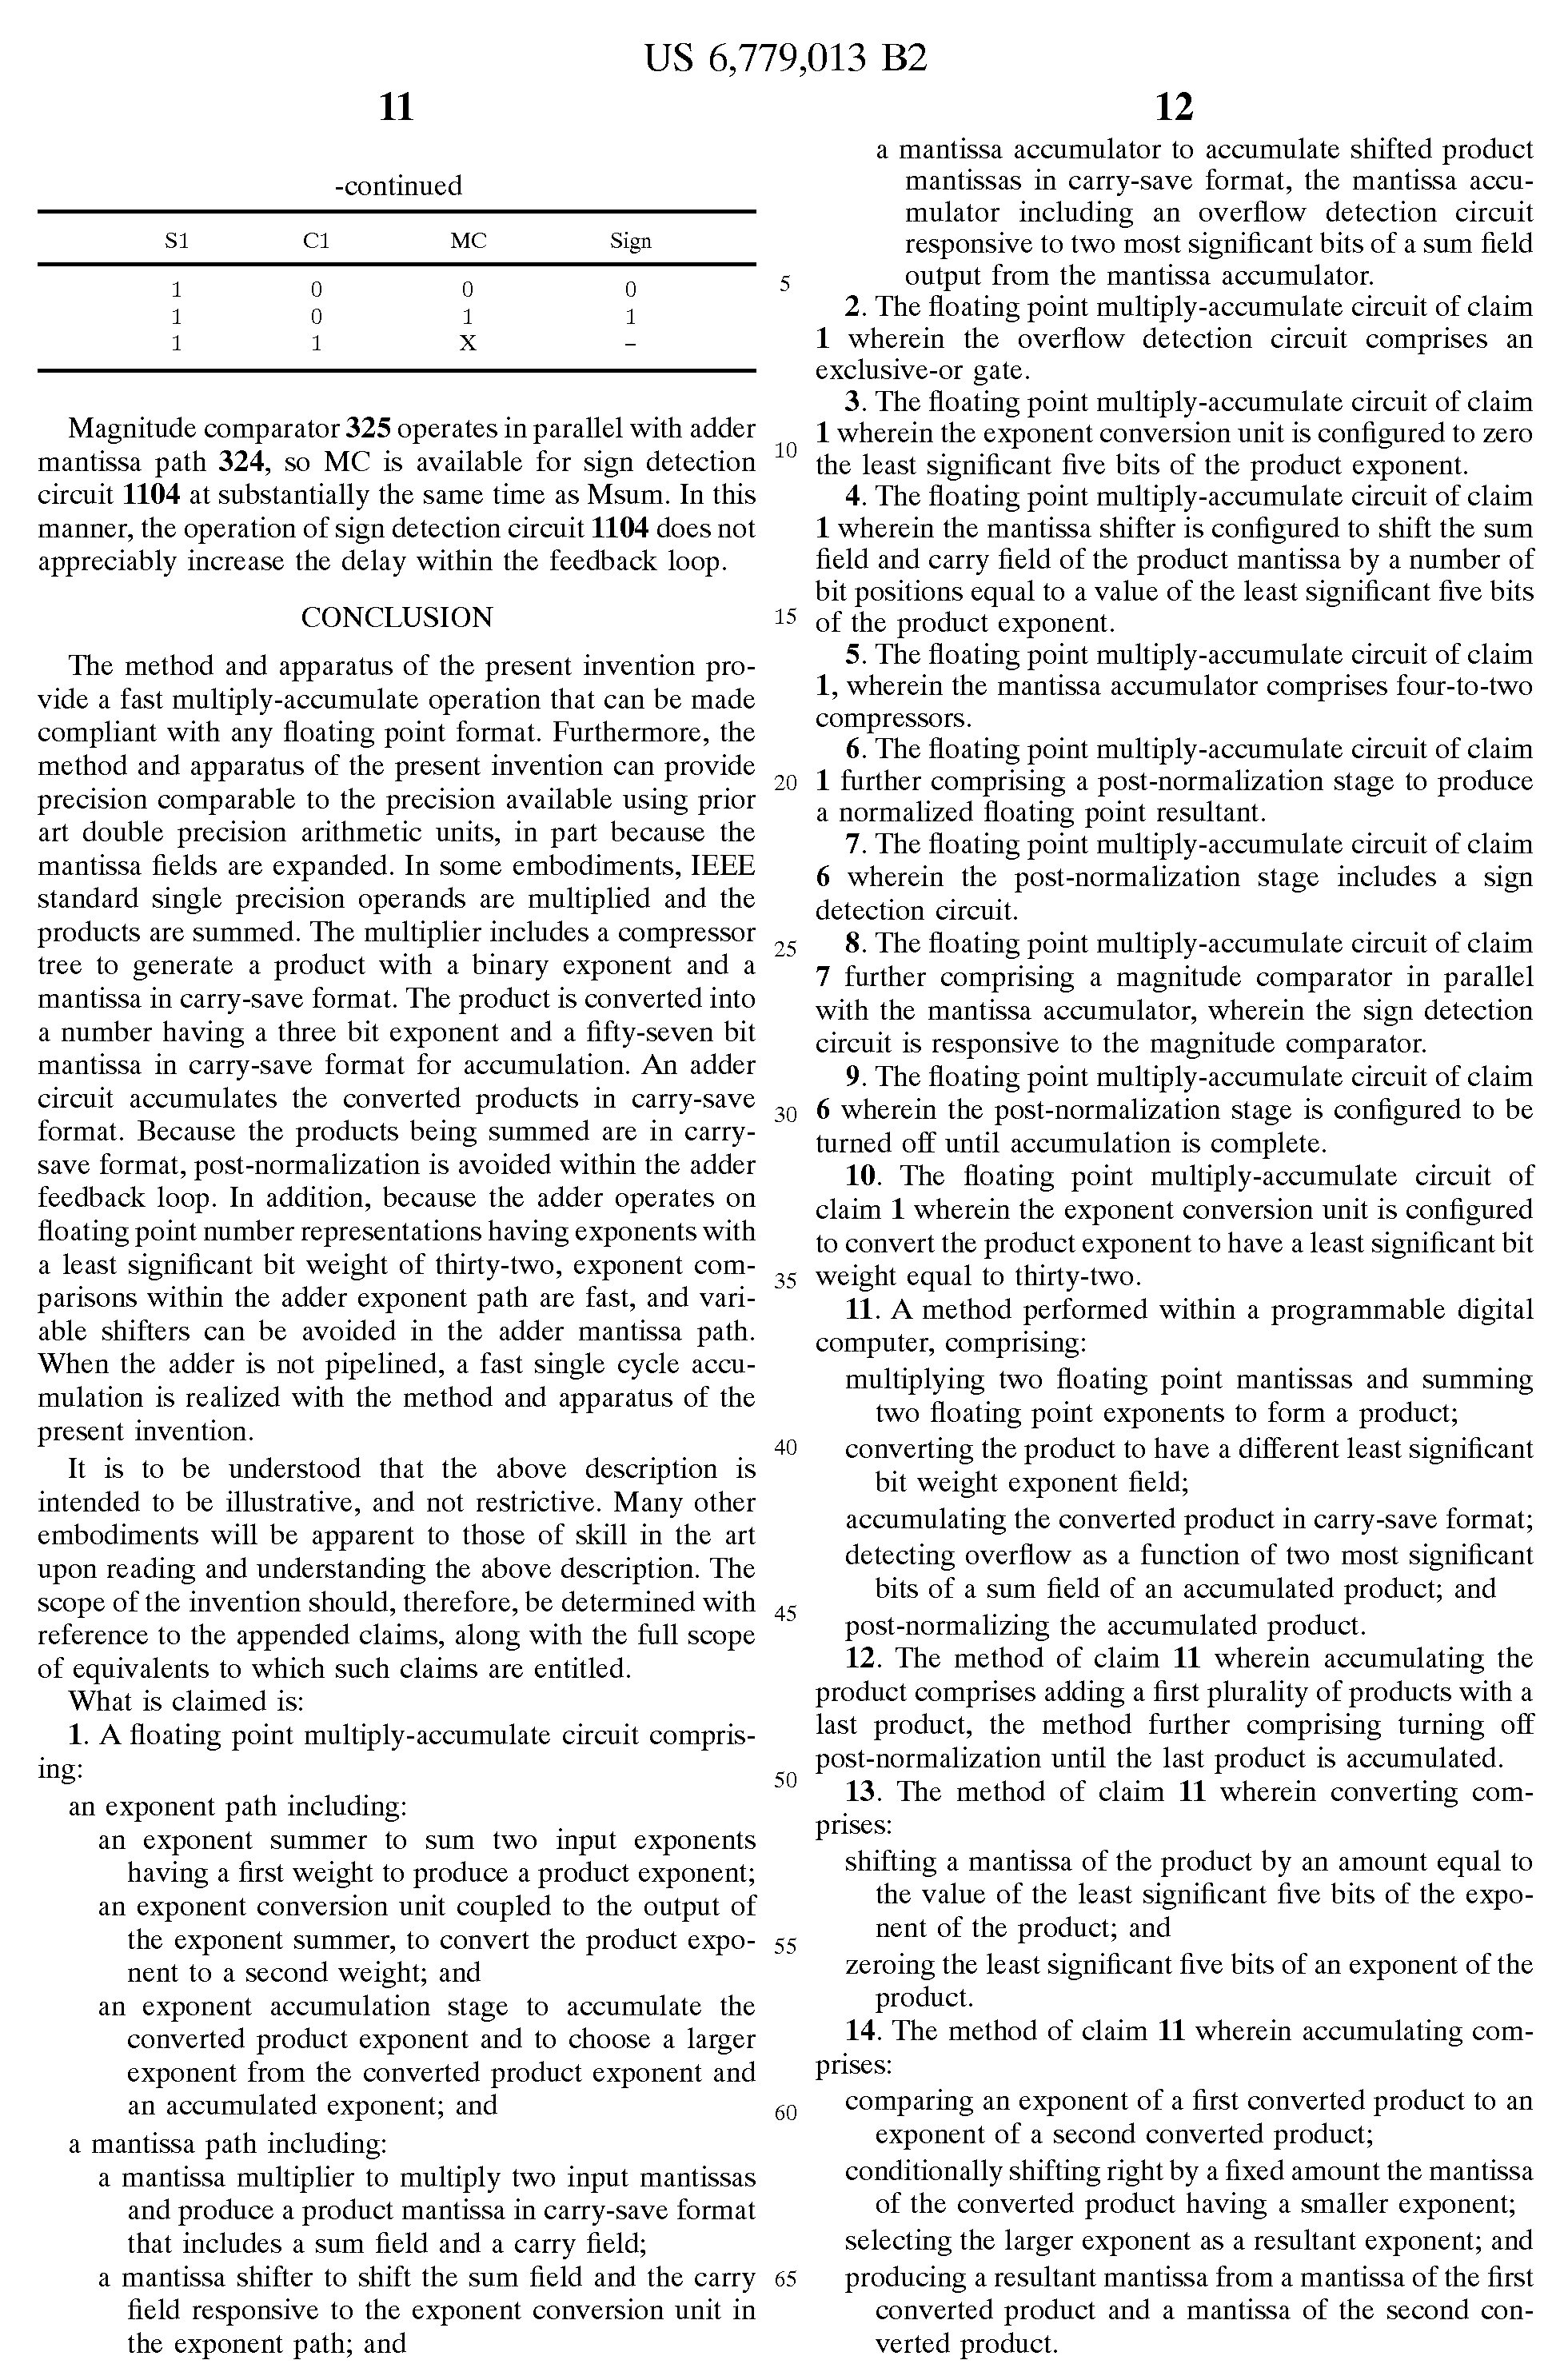
\includegraphics[width=0.89444in,height=0.27778in]{vertopal_51ee0767b0954baa94830c5e62d37958/media/image3.png}

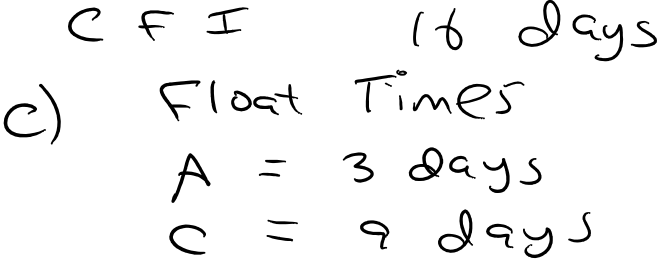
\includegraphics[width=0.18056in,height=0.46944in]{vertopal_51ee0767b0954baa94830c5e62d37958/media/image4.png}

2

\textbf{5.Describe the main differences between the VLSI and embedded
system design} \textbf{processes. {[}A{]}}

\begin{quote}
VLSI and embedded systems design share similarities and contain
differences. They are both similar in that they have phases for
requirements specifications, system architecture design, and technical
design. The difference between them lies in the technical design, where
the steps depend upon the technology that is being developed. In the
case of VLSI, steps are used to successively refine the design to meet
develop a layout level circuit; however, embedded design requires that
the technical design phase consists of software and hardware co-design.
\end{quote}

\textbf{6.Using the library or Internet, conduct research on the spiral
software design process. What are the advantages and disadvantages of
this relative to the waterfall model? Be sure to cite references.
{[}A{]}}

\begin{quote}
The spiral methodology reflects the relationship of tasks with rapid
prototyping, increased parallelism, and concurrency in design and build
activities.1 The spiral process recognizes that errors will occur in all
stages of the production process and proceeds on this basis.2 It is
agreed that the development processes will have to be revisited multiple
times as the design furthers completion; therefore, unlike the Waterfall
model, this methodology incorporates an iteration cycle, which is
continued until the design is fully complete. A Spiral Development Model
diagram can be found at \uline{http://www.hyperthot.com/pm\_sdm.htm} as
well at other sites on the Internet.

Embedded in spiral design is the process of refactoring -- changing
software in such a way as to improve structure, but not affect the end
result.3 Overall, the spiral software design model is not as rigid,
concrete, and strict as the Waterfall model; however, this method should
still be planned methodically, with tasks and deliverables identified
for each step within the spiral. The table below lists the advantages
and disadvantages of the spiral design model in reference to the
waterfall model.
\end{quote}

1 Chapman, James. ``Spiral Methodology.'' \emph{Software Development
Methodology.} 2005. 20 May 2005

\begin{quote}
\textless{} http://www.hyperthot.com/pm\_sdm.htm \textgreater.
\end{quote}

2 Culwin, Fintan. ``The Production Process.'' \emph{LAW -- Learn Ada On
the Web}. 1998. 20 May 2005

\textless{} http://www.scism.sbu.ac.uk/law/Section1/chap1/s1c1p3.html
\textgreater{}\\
3 Hean, Daniel. ``Design through to testing.'' \emph{Content \& Document
Management System.} 2005. 20 May 2005.

\begin{quote}
\textless{}
http://www.yedit.com/web-content-management-system/400-design-through-to-testing.html
\textgreater{}
\end{quote}

3

\begin{longtable}[]{@{}
  >{\raggedright\arraybackslash}p{(\columnwidth - 6\tabcolsep) * \real{0.2500}}
  >{\raggedright\arraybackslash}p{(\columnwidth - 6\tabcolsep) * \real{0.2500}}
  >{\raggedright\arraybackslash}p{(\columnwidth - 6\tabcolsep) * \real{0.2500}}
  >{\raggedright\arraybackslash}p{(\columnwidth - 6\tabcolsep) * \real{0.2500}}@{}}
\toprule()
\begin{minipage}[b]{\linewidth}\raggedright
\end{minipage} & \begin{minipage}[b]{\linewidth}\raggedright
\begin{quote}
Advantages
\end{quote}
\end{minipage} & \begin{minipage}[b]{\linewidth}\raggedright
\end{minipage} & \begin{minipage}[b]{\linewidth}\raggedright
\begin{quote}
Disadvantages
\end{quote}
\end{minipage} \\
\midrule()
\endhead
1 & \begin{minipage}[t]{\linewidth}\raggedright
\begin{quote}
Increased time-to-market
\end{quote}
\end{minipage} & \begin{minipage}[t]{\linewidth}\raggedright
\begin{quote}
1
\end{quote}
\end{minipage} & \begin{minipage}[t]{\linewidth}\raggedright
\begin{quote}
Revisiting the same stages
\end{quote}
\end{minipage} \\
2 & \begin{minipage}[t]{\linewidth}\raggedright
\begin{quote}
Incremental \& Iterative
\end{quote}
\end{minipage} & \begin{minipage}[t]{\linewidth}\raggedright
\begin{quote}
2
\end{quote}
\end{minipage} & \begin{minipage}[t]{\linewidth}\raggedright
\begin{quote}
Requirements are not fully identified
\end{quote}
\end{minipage} \\
3 & \begin{minipage}[t]{\linewidth}\raggedright
\begin{quote}
Promotes increase in documentation
\end{quote}
\end{minipage} &
\multirow{6}{*}{\begin{minipage}[t]{\linewidth}\raggedright
\begin{quote}
3
\end{quote}
\end{minipage}} &
\multirow{6}{*}{\begin{minipage}[t]{\linewidth}\raggedright
\begin{quote}
Project goal is not initially established
\end{quote}
\end{minipage}} \\
4 & \begin{minipage}[t]{\linewidth}\raggedright
\begin{quote}
No set structure or phase routine
\end{quote}
\end{minipage} \\
5 & \begin{minipage}[t]{\linewidth}\raggedright
\begin{quote}
Non-idealistic
\end{quote}
\end{minipage} \\
6 & \begin{minipage}[t]{\linewidth}\raggedright
\begin{quote}
Not as costly to revisit process steps
\end{quote}
\end{minipage} \\
7 & \multirow{2}{*}{\begin{minipage}[t]{\linewidth}\raggedright
\begin{quote}
Primitive to more intricate design\\
Allows development to begin w/o full understanding
\end{quote}\strut
\end{minipage}} \\
8 \\
\bottomrule()
\end{longtable}

\textbf{7.Using the library or Internet, conduct research on the Extreme
Programming design} \textbf{process. Outline the significant elements of
the Extreme Programming paradigm. What} \textbf{are the pro and con
arguments for this software development model? Be sure to cite}
\textbf{references. {[}A{]}}\\
Extreme Programming is a methodology -- although it's debatable - of
programming that was started back in the early 1990's by Kent Beck. Beck
realized that there were four key components, or dimensions, that were
crucial for the success of a software project -- \textbf{communication},
\textbf{simplicity}, \textbf{feedback}, and \textbf{courage}. One can
view extreme programming as a streamlined software development process
that focuses on delivering software when needed.4\\
Characteristics of Extreme Programming\\
•Needs identification -- get ``stories'' from user on what they want the
software to do.

\begin{quote}
•Small teams of programmers.

•Many iterations. The team develops code and shows it to the client
early to see if it satisfies and changes as necessary.

•Much early testing.

•Agreed upon coding standards are followed.

•ALL code is written by two people working together!

•Continuous Testing. All code is test early on -- has test plan
integrated with coding •Coders work no more than 40 hour/ wee.

•Teamwork is encouraged and very important.
\end{quote}

4Wells, Don. "The XP Philosophy." \emph{XP Extreme Programming}. 1999.

\begin{quote}
Extreme Programming. 8 Sep. 2004 \textless{}
http://www.extremeprogramming.org/Kent.html \textgreater.
\end{quote}

4

\begin{quote}
•Refactoring. Factor out duplicate code.

The current practices of an XP (Extreme Programmer) are subdivided into
12 arenas. These

subdivisions are The Planning Game, Small Releases, System Metaphor,
Simple Design,

Continuous Testing (Unit and Acceptance), Refactoring, Pair Programming,
Collective Code

Ownership, Continuous Integration, 40-hour Work Week, On-site Customer,
and Coding

Standards.5 Each of these practices is precisely defined; however,
merely mentioning them

is adequate for the task at hand. A flow of the Extreme Programming
process can be

accessed via http://www.extremeprogramming.org/ map/project.html.6 and
at other locations

on the Internet.

The idea of XP seems very promising. There are some clear advantages to
this style and

method of programming. However, there are some very distinct
disadvantages also. The

table below lists all the advantages and disadvantages of this fairly
new style of

programming.
\end{quote}

\begin{longtable}[]{@{}
  >{\raggedright\arraybackslash}p{(\columnwidth - 2\tabcolsep) * \real{0.5000}}
  >{\raggedright\arraybackslash}p{(\columnwidth - 2\tabcolsep) * \real{0.5000}}@{}}
\toprule()
\begin{minipage}[b]{\linewidth}\raggedright
\begin{quote}
Advantages
\end{quote}
\end{minipage} & \begin{minipage}[b]{\linewidth}\raggedright
\begin{quote}
Disadvantages
\end{quote}
\end{minipage} \\
\midrule()
\endhead
\bottomrule()
\end{longtable}

\begin{quote}
1 Stresses customer satisfaction 1 Like a jigsaw puzzle (lack of
structure)

2 Enables groupware style development 2 Departure from traditional
methods

3 Saving money (reduce software costs) 3 Pair programming

4 Thorough testing 4 Source code hard to understand/maintain

5 Lightweight methodology (few rules) 5 Flaws with YAGNI philosophy

6 Delivers software when needed ("You Aren\textquotesingle t Gonna Need
It")

7 Doesn\textquotesingle t overdesign desired system 6 Overlooks
organizational problems

Overall, XP has many great ideas for improving efficiency and
productivity; however, it still

contains serious structural issues that could prove counterproductive.

\emph{\textbf{Note:} We find this (and previous problem) to be a
valuable exercise because it}

\emph{demonstrates to students that design processes are evolving and
important. The pitfall of}

\emph{many is to not follow a process and just try to proceed directly
to a solution.}
\end{quote}

\textbf{8.Project Application. In preparation for the project and team
selection, develop a}

\begin{quote}
\textbf{personal inventory that includes a list of five favorite
technologies or engineering}

\textbf{subjects that you are interested in pursuing. Also, list the
strengths and weaknesses that}

\textbf{you bring to a project team. {[}P{]}}
\end{quote}

5Brewer, John. "Extreme Programming FAQ." \emph{Extreme Programming
(XP)}. 2001.

\begin{quote}
9 Sep. 2004 \textless{}
http://www.extremeprogramming.org/rules/iterative.html \textgreater.
\end{quote}

6Wells, Don. "Iterative Development." \emph{XP Extreme Programming}.
1999.

\begin{quote}
Extreme Programming. 9 Sep. 2004
\textless http://www.extremeprogramming.org/rules/iterative.html
\textgreater.
\end{quote}

5

\begin{quote}
\emph{\textbf{Note:} We find this exercise an important step in starting
students on the path of team formation and project selection and usually
assign it on the first day of class. We setup an electronic bulletin
board for the students and have them post this information publicly for
the whole class to see. Students are then encouraged to review this and
identify potential team-mates. We have also done a variation where each
student is required to determine this information and then make a short
oral presentation (2 minute pitch) to the class, in which they describe
what types of projects they are interested in and what strengths/skills
they can bring to a team.}
\end{quote}

6

\end{document}
